\begin{appendices}

\section{Much longer words}
\label{app:much_longer}

\begin{minipage}{\textwidth}
        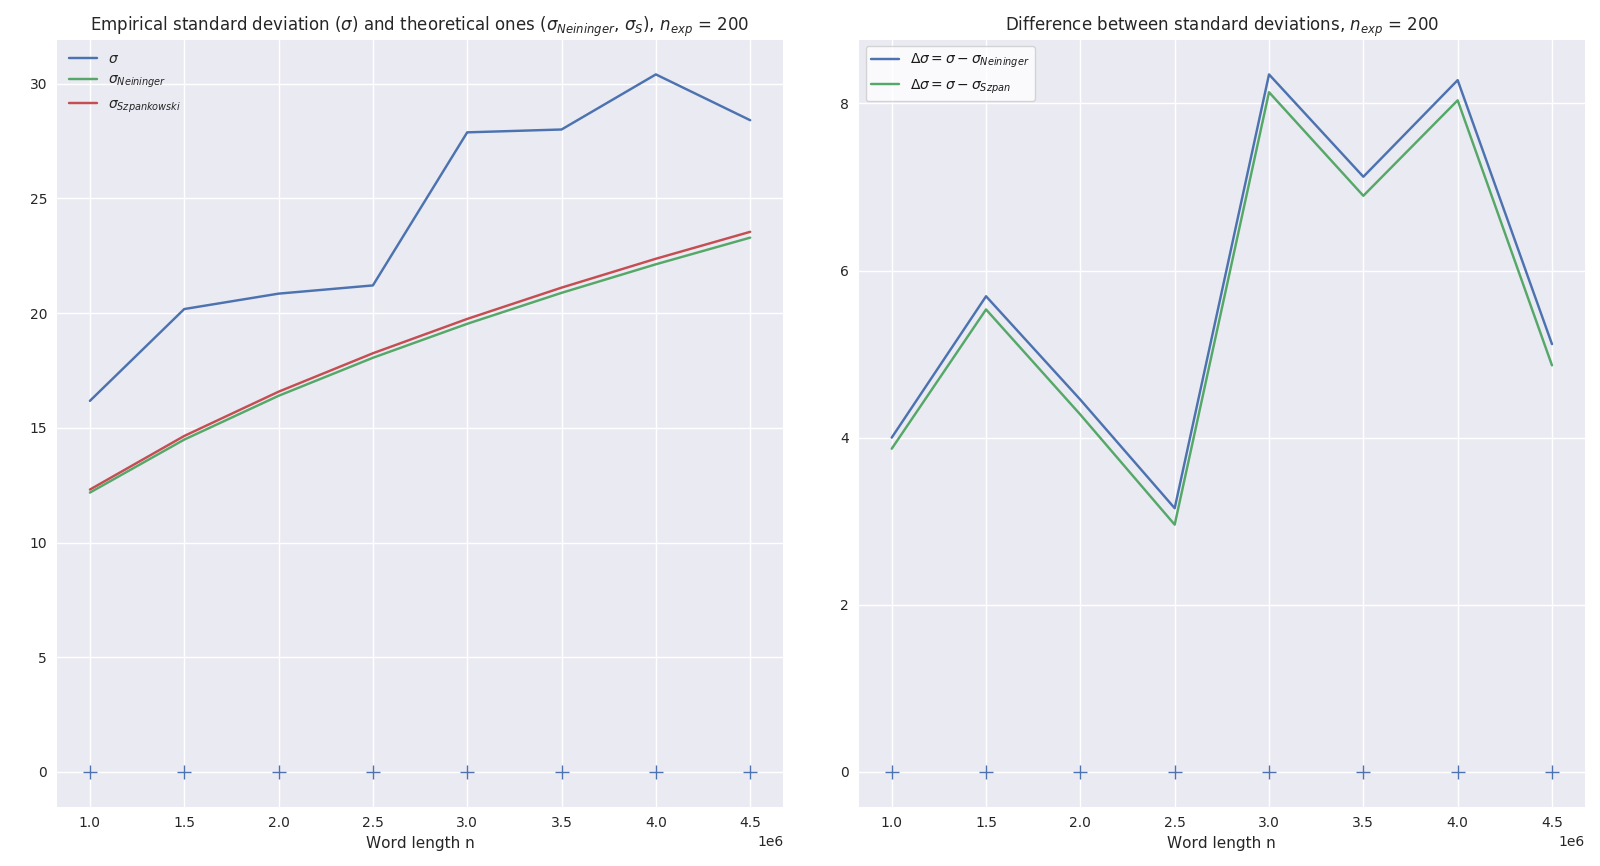
\includegraphics[width = \textwidth,
        				    trim = 0 0 0 0,
        				    	clip=true]{./figs/eig_fig5.png}	
	\end{minipage} 

\noindent
 	 \begin{minipage}{\textwidth}
        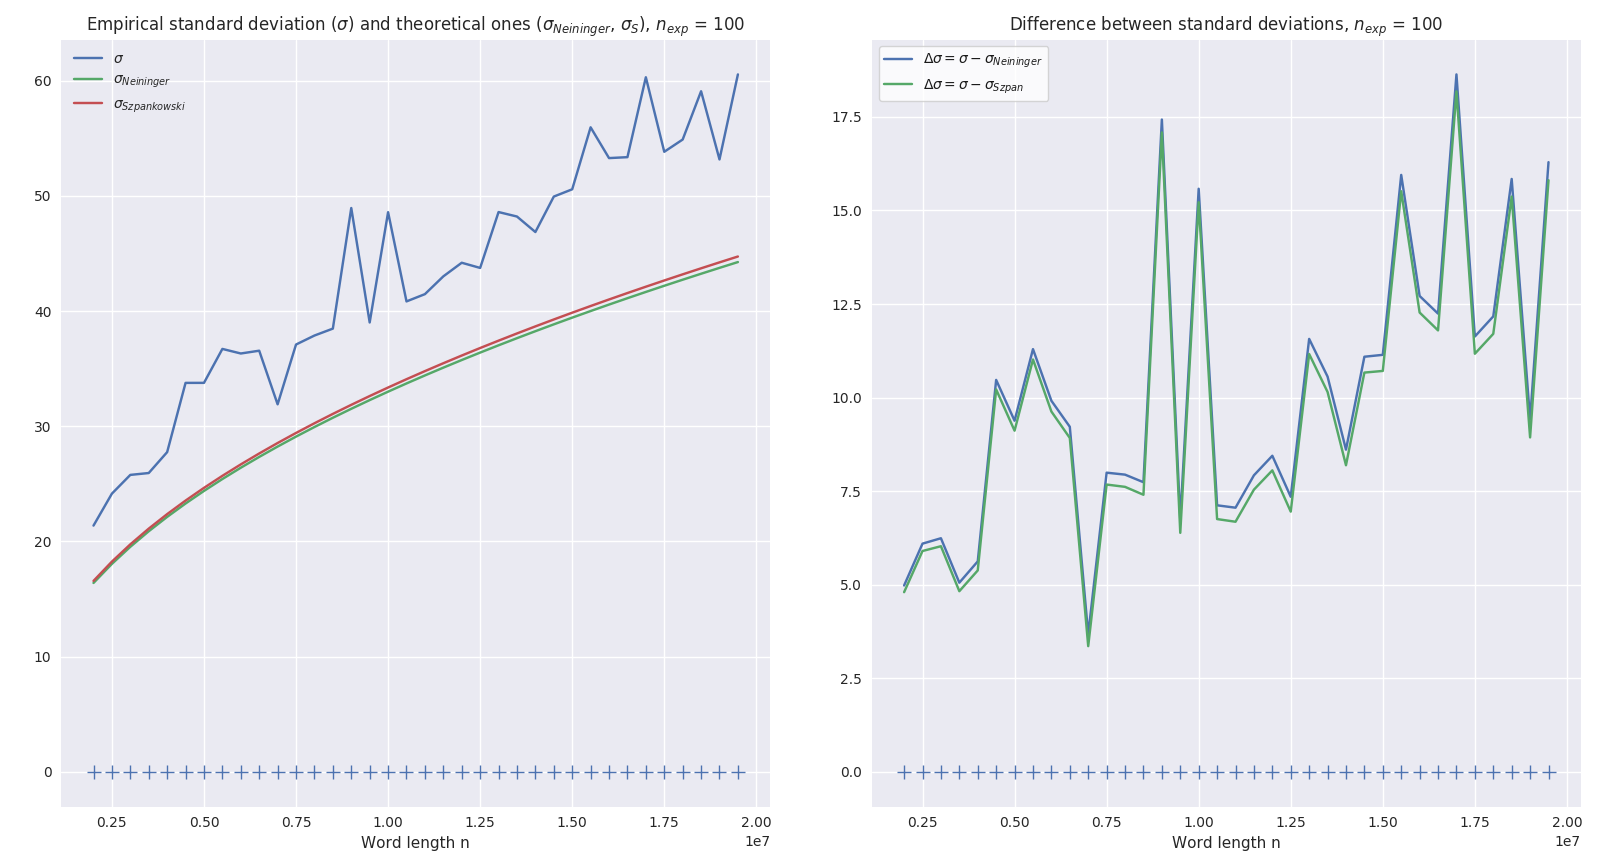
\includegraphics[width = \textwidth,
        				    trim = 0 0 0 0,
        				    	clip=true]{./figs/eig_fig4.png}	
	\end{minipage} 

\pagebreak
\section{Another (more complicated) computation of $\ddot{\lambda}(-1)$}
\label{app:comp_lam1}
This expression gives the sames numerical results as the first one, 
but is more complex to compute for no apparent gain other than having 
yet another similar way of computing $\ddot{\lambda}(-1)$. 
Computing $\delta(s)$, a complex root of 
$\Delta(s)$, writing $\Delta$ as :

\begin{calculs}
    & \Delta 
        &=& \underbrace{p_{0 0}^{-2\Re(s)} \cos(2\ln(p_{0 0})\Im(s))}_{a_0(s)} \\[6mm]
          &&+& \underbrace{p_{1 1}^{-2\Re(s)} \cos(2\ln(p_{1 1})\Im(s))}_{a_1(s)} \\[6mm]
           &&& \underbrace{- 2 (p_{0 0}\,p_{1 1})^{-\Re(s)} \cos(\ln(p_{0 0}\,p_{1 1})\Im(s))}_{a_2(s)} \\[6mm]
           &&+&  \underbrace{4 (p_{0 1}\,p_{1 0})^{-\Re(s)} \cos(\ln(p_{0 1}\,p_{1 0})\Im(s))}_{a_3(s)} \\[6mm]
          &&+& i \Im(\Delta) 
\end{calculs}

where $\Im(\Delta) = b_0(s) + b_1(s) + b_2(s) + b_3(s)$, with each $b_i(s)$ being
the same term as $a_i(s)$ with $\cos$ replaced by $\sin$. Writing

\centers{$\Delta = \alpha(s) + i \beta(s)$}

and searching for $\delta = x(s) + i y(s)$, meaning that

\centers{$ \left\{
                \begin{array}{rl}
                    x^2 - y^2 &= \alpha \\
                    2\, x\, y &= \beta \\
                    x^2 + y^2 &= \sqrt{\alpha^2+\beta^2}
                \end{array}
            \right.
        $}
    

This yields
 
    \centers{$
        \left\{
            \begin{array}{rl}
                     x &= \pm \sqrt{\f{1}{2}(\sqrt{\alpha^2+\beta^2}+\alpha)} \\
                     y &= \pm \sqrt{\f{1}{2}(\sqrt{\alpha^2+\beta^2}-\alpha)} 
            \end{array}
        \right. 
            $}

and since $2xy = \beta$, there is $\epsilon \in \{-1,1\}$ such that
             \centers{$ \delta = \pm (x + \ir \epsilon y) $}

\leftcenters    
    {so}
    {$\lambda(s) = \f{ \poo + \pii \pm (x + \ir \epsilon y)}{2}$}

\leftcenters
    {\text{i.e.}}
    {$\ddot{{\lambda}}(-1) = \f{ p_{0 0} \ln^2(p_{0 0})
                                    + p_{1 1} \ln^2(p_{1 1})
                                    \pm (\ddot{{x}}(-1) + \ir \epsilon \ddot{{y}}(-1))}
                                  {2} $}
where we'll have to find what is $\epsilon$ and which sign to pick.

But first, computing the derivatives of $x(s) = \sqrt{f(s)} $:
    \centers{$\dot{x}(s) = \f{f'(s)}{2x(s)}$}
    \leftcenters
        {and}
        {$\ddot{{x}}(s) = \f{ f''(s) x(s) - f'(s) \cdot \f{f'(s)}{2x(s)} }
                                   { 2 x^2(s) } $}

and then computing $f(s)$ :

    \centers{$ f(s) = \f12 (\sqrt{\alpha^2+\beta^2} + \alpha) $}
    \centers{$ f'(s) = \f12 \left[ \f{ \overbrace{ \dot{\alpha}\alpha + \dot{\beta}\beta }^{ \gamma(s) } }
                                     { \underbrace{\sqrt{\alpha^2 + \beta^2}}_{\kappa(s)} }
                                    + \dot{\alpha} \right] $}

    \leftcenters{with}{$ \dot{\alpha} = \dot{a_0} + \dot{a_1} + \dot{a_2} + \dot{a_3} $}

\leftcenters
    {As for $f''(s)$, it is}
    {$ f''(s) = \f12 \left[ 
                        \f{ \dot{\gamma}(s) \kappa(s) - \gamma(s) \dot{\kappa}(s) }
                          {\kappa^2(s)} 
                        + \ddot{{\alpha}}(s) 
                    \right] $}

\leftcenters
    {with}
    {$\dot{\gamma}(s) = \ddot{{\alpha}} \alpha + {\dot{\alpha}}^2 + \ddot{{\beta}}\beta + {\dot{\beta}}^2$}

\centers
    {$ \dot{\kappa}(s) = \f{2 \alpha \dot{\alpha} + 2 \beta \dot{\beta}}
                           {2\sqrt{\alpha^2+\beta^2}}$}


Derivating according to $s$ amounts to derivating according to $\Re(s)$, so in $s=-1$ :

    \centers{$ \dot{\alpha}(-1) = -2\ln p_{0 0} a_0(-1)
                              -2\ln p_{1 1} a_1(-1)
                              -\ln q_0 a_2(-1)
                              -\ln q_1 a_3(-1) $}
\leftcenters
    {and}
    {$ \ddot{\alpha}(-1) = 4\ln^2 p_{0 0} a_0(-1)
                             + 4\ln^2 p_{1 1} a_1(-1)
                              +\ln^2 q_0 a_2(-1)
                              +\ln^2 q_1 a_3(-1) $}

At this point we have fully determined $\ddot{{x}}(s)$, and we realize two things:

\begin{enumerate}
    \item In $s=-1$, since $Im(-1) =0$ and because of the sinus function,
          all the $\beta$ terms, including derivatives, are equal to 0.
          This will simplify the expression for $\ddot{{x}}(-1)$. \\

    \item Furthermore, it also means that $\ddot{{y}}(-1) = 0$,
          so
          \encadre{ $\ddot{{\lambda}}(-1) = \f{ p_{0 0} \ln^2(p_{0 0})
                                    + p_{1 1} \ln^2(p_{1 1})
                                    + \ddot{{x}}(-1) }
                                  {2} $ }
          where the $+$ comes from the fact that $\lambda(s)$ is 
          the highest eigenvalue (and $\ddot{{x}}(-1) > 0$, so by
          continuity the expression around $s=-1$ retained the same sign)
\end{enumerate}

The final expression of $\ddot{{\lambda}}$ (as well as $\dot{\lambda}(-1))$)
can be fully expressed with $\alpha(-1), \dot{\alpha}(-1)$ and $\ddot{{\alpha}}(-1)$.
I empirically verified that $\dot{\lambda}(-1) = h$, and the final result is the same
as with the first method of computation.


% \pagebreak
% \section{Code for computing $\ddot{lambda}(-1)$}
% \label{app:comp_lam2}
% \lstinputlisting[firstline=156,lastline=206]{../src/eigenvalues.py}



\end{appendices}